\documentclass[10pt,a4paper]{article}
\usepackage[latin1]{inputenc}
\usepackage{amsmath}
\usepackage{amsfonts}
\usepackage{amssymb}
\usepackage{float}
\usepackage{graphicx}
\begin{document}
\section{Descripci�n del problema.}
\section{Datos.}
\section{Herramientas.}
Las herramientas que se pueden usar para abordar la resoluci�n del problema es amplia. Es por ello, que resulta dif�cil elegir la m�s adecuada. Tras un estudio de las bibliotecas disponibles para los distintos lenguajes de programaci�n que domino, me seleccione weka(java),sklearn(python) y R. Para determinar cual de las 3 es la m�s conveniente en este caso, realizar� pruebas de ejecuci�n de los diferentes algoritmos y compararemos el tiempo de ejecuci�n y el uso de memoria. Adem�s, se debe tener en cuenta la facilidad para tratar los datos tanto para su lectura, como para la generaci�n de los archivos con las predicciones. 

Los resultados obtenidos se muestran en las siguientes gr�ficas:	
\begin{figure}[!h]
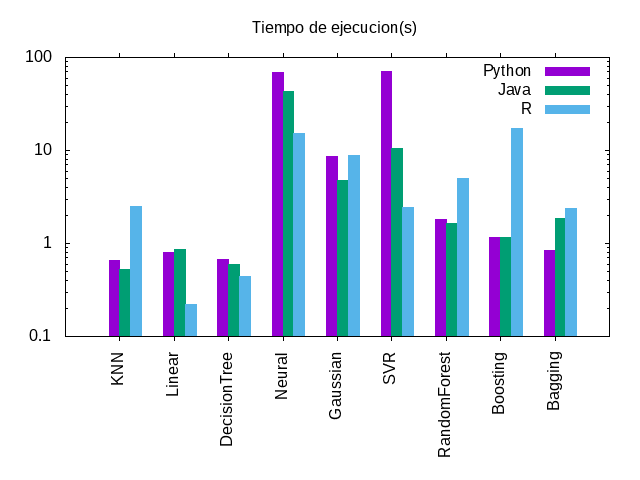
\includegraphics[scale=0.75]{./img/tiempos.png}
\caption{Test algoritmos:Tiempo de ejecucion}
\end{figure}
\begin{figure}[H]
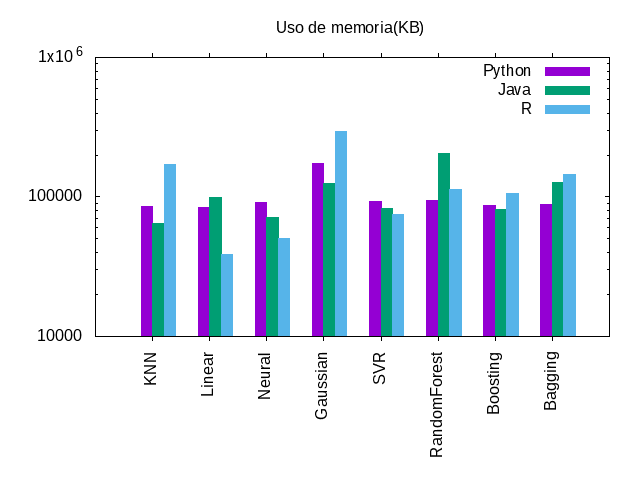
\includegraphics[scale=0.75]{./img/memoria.png}
\caption{Test algoritmos:Memoria usada}
\end{figure}

Observando los resultados podemos concluir que sklearn y weka ofrecen (en media) un rendimiento similar, mientras que R ofrece un mejor rendimiento para los algoritmos b�sicos pero es inferior en la ejecucion de multiclasificadores.
Por otro lado, R y sklearn permiten tratar los datos de forma c�moda. Otra cuesti�n a tener en cuenta, es la buena documentaci�n con la que cuenta sklearn. 


En conclusi�n, el lenguaje a usar ser� Python ya que permite un manejo de los datos flexible y un c�digo legible propio de este lenguaje. Esta decisi�n se apoya en que en t�rminos de rendimiento no hay una alternativa "mucho mejor".

En particular, se usaran las siguientes bibliotecas:
\begin{itemize}
\item NumPy.
\item Pandas.
\item Scikit Learn.
\item XGBoost.
\end{itemize}
\section{Algoritmos.}
\textbf{Nota: Para la ejecucion de los algoritmos los datos nominales se han pasado a numerico.}

A priori desconocemos que algoritmo se adapta mejor a nuestro problema, es por ello que realizaremos un estudio comparando varios algoritmos. Los algoritmos elegidos son los siguientes:
\begin{itemize}
	\item algoritmos b�sicos como KNN,Linear Regression y Arboles de regresion
	\item  algoritmos "potentes" como NeuralNetwork,Gaussian y SVM
	\item multiclasificadores como Random Forest, Boosting y Bagging
\end{itemize} En la siguiente gr�fica se muestran los resultados obtenidos.
\begin{figure}[H]
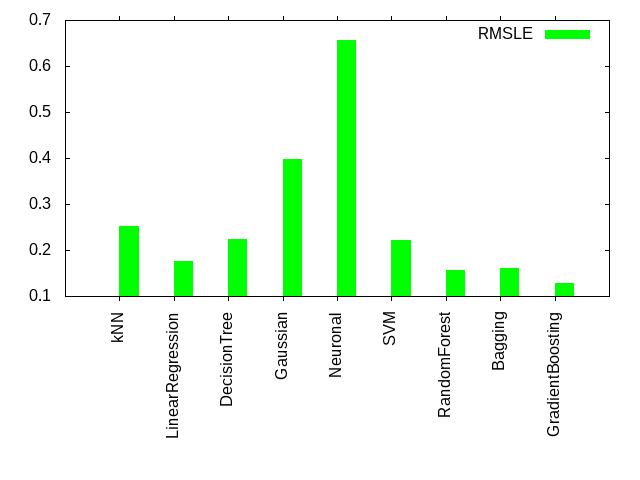
\includegraphics[scale=0.75]{./img/error.png}
\caption{Test algoritmos:Error.}
\end{figure}
Se puede observar que los algoritmos que mayor precision proporcionan en este caso son los multiclasificadores. Por tanto, al igual que los competidores, nos decantamos por esta opci�n.
\end{document}